\section{Architecture}

\subsection{Stakeholders}

\subsubsection{Customer}
Our goal with this course is to make a product that work as the customer intended but also performs satisfactorily. The code we're writing needs to be written following the clean coding standard and use interfaces/polymorphy so their developers can further develop this solution.

\subsubsection{Course Evaluator}
The course evaluator needs to be satisfied if we want a good grade, that means that we need to satisfy all the other stakeholders and deliver a well documented report of everything.

\subsubsection{Supervisor}
The supervisor said in the first meeting that he would fight for our grade given that he was satisfied. This means that we should complete the project deliver a well documented report. \\ We should also take advices from him, especially when there's issues among us in which we need to tell the supervisor so he can help solve the issue.
\subsubsection{Implementers}
The architecture should be easy to implement and make sense to the coders.

\subsection{Quality Attributes}
The customer was very specific when it came to what they wanted.
\subsubsection{Modifiability}
The solution we're making will be used for other ads than real estate ads, therefore we need to make it modifiable so other developers later on can further develop using our solution as a base.
\subsubsection{Performance}
We want the system to perform with a satisfactory performance.
\subsubsection{Availability}
The system should be available for the users when they need it.
\subsubsection{Interoperability}
Needs to inter-operate with already-existing order system, this will be done by using the technology the customer tells us to use; Web-api, mssql etc...
\subsubsection{Readability}
The customer wants us to write readable code. We are supposed to do a polymorphy/interface type of programming so it's easier for other developers to extend via plugins etc. therefore it's important that the code is readable so other's can easily understand what's going on without much hazzle.

\subsection{Views}


\subsubsection{Process view}
There is no need for us to supply a process view, because we do not have access to their server. We are only supposed to write the code for their system, without taking into account how the processes interoperate.
\subsubsection{Logical view}
\begin{figure}[h]
\centering
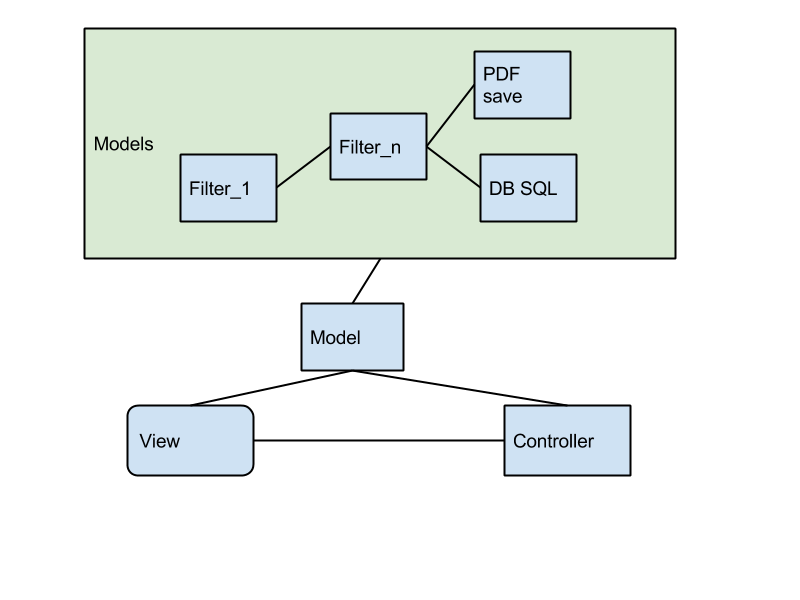
\includegraphics[width=0.8\textwidth]{images/architecture00.png}
\caption{Logical view}
\label{fig:logical_view}
\end{figure}
\newpage

\subsubsection{Scenario view}
\begin{figure}[h]
\centering
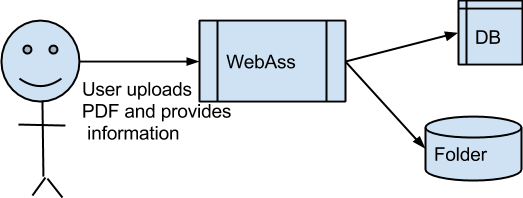
\includegraphics[width=0.8\textwidth]{images/architecture01.png}
\caption{Scenario view}
\label{fig:scenario_view}
\end{figure}


\subsubsection{Physical view}
\begin{figure}[h]
\centering
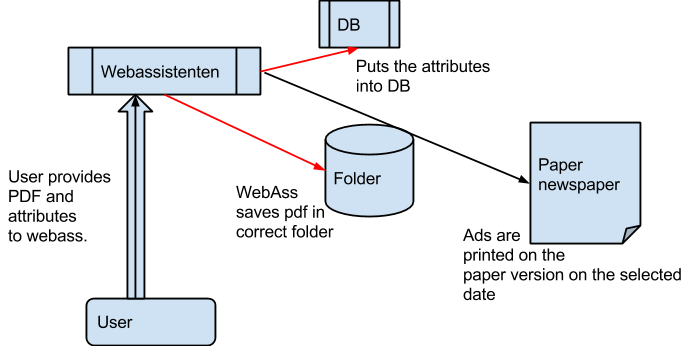
\includegraphics[width=0.8\textwidth]{images/architecture02.png}
\caption{Physical view, we implement the red arrows}
\label{fig:physical_view}
\end{figure}
\newpage
\subsection{Class diagram}
From these views, we made this class diagram.
\begin{figure}[h]
\centering
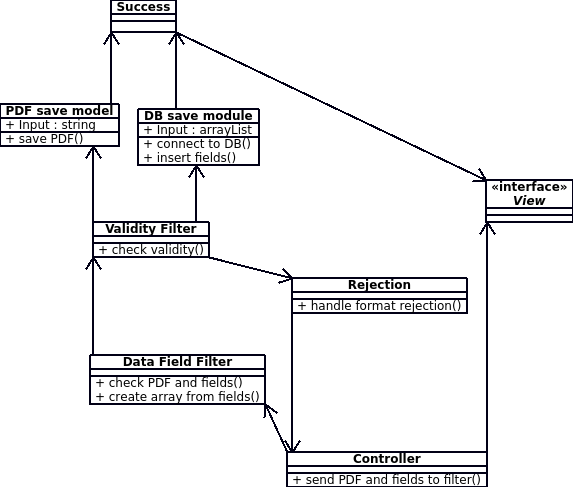
\includegraphics[width=0.8\textwidth]{diagrams/class_diagram.png}
\caption{Digital class diagram}
\label{fig:class_diagram}
\end{figure}
\subsection{Patterns}
MVC due to the technology and pipe \&  filter to filter the data and due to the modifiability requirement.
\subsection{Tactics}
\subsubsection{Modifiability}
\begin{itemize}
\item Increase semantic cohesion
\item Decrease coupling
\item Split modules
\end{itemize}

\subsubsection{Performance}
\begin{itemize}
\item Write optimal code
\end{itemize}

\subsubsection{Availability}
\begin{itemize}
\item Our code should not crash the customer's system, but it's their responsibility that the system is available.
\end{itemize}

\subsubsection{Interoperability}
\begin{itemize}
\item The technology and tools we're using should be sufficient to ensure interoperability
\end{itemize}

\subsubsection{Readability}
\begin{itemize}
\item We will follow the clean coding principle and use camelCase coding. Refer to the Templates and Standards section.
\end{itemize}